\documentclass[../report.tex]{subfiles}

\begin{document}
% --------------------------------------------------------------------------
% SECTION 2 
% --------------------------------------------------------------------------
\section{State space control (LQG) of stable aircraft}
\subsection{Creation and description of the model}

\begin{figure}[h]
    \centering
    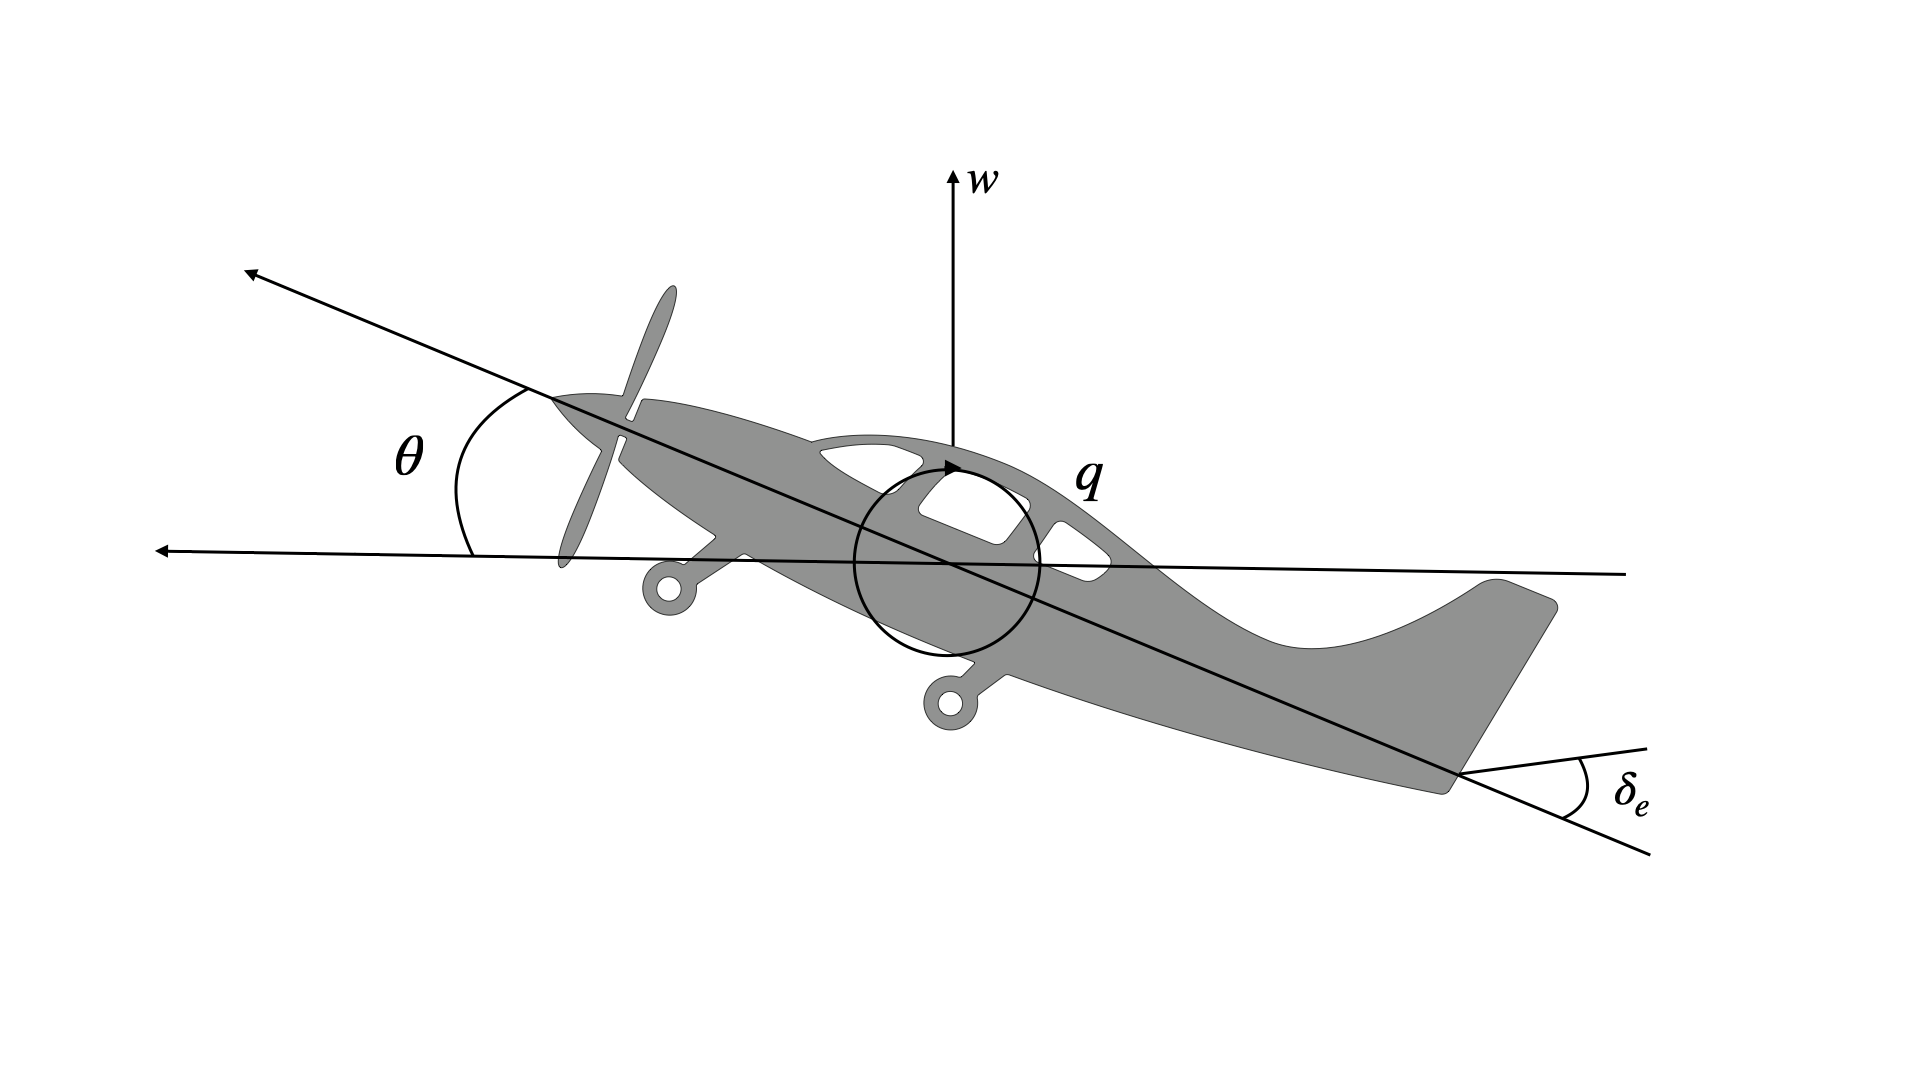
\includegraphics[width=0.6\textwidth]{aircraft.png}
    \caption{Aircraft longitudinal motion.}
    \label{fig:aircraft}
\end{figure}

\begin{tabular}{ |c|c| }
    \hline
    $\beta$ & Sideslip angle \\
    $p$ & Roll rate\\
    $r$ & Yaw rate\\
    $\Phi$ & Roll angle\\
    $w$ & Vertical velocity\\
    $q$ & Pitch rate\\
    $\theta$ & Pitch angle\\
    $\delta_e$ & Elevator deflection\\
    \hline
\end{tabular}

TODO: More about the system model. \\

The dynamic model of the aircraft system \ref{fig:aircraft} is taken from
the article \cite{air_lqg}.
For longitudinal motion:
\begin{equation}
    \beta = p = r =\Phi = 0
\end{equation}
The transfer function is represented in state-space form by matrices:
\begin{align} \label{sys_ss}
    \begin{split}
        \dot{x} &= Ax + Bu \\
        y &= Cx + Du
    \end{split}
\end{align}

$A = \begin{bmatrix} -0.3149 & 235.8928 & 0 \\
                     -0.0034 & -0.4282  & 0 \\
                      0      & 1        & 0 \end{bmatrix}$ \\


$B = \begin{bmatrix} -5.5079   \\
                      0.0021   \\
                      0        \end{bmatrix}$ \\


$C = \begin{bmatrix}  0 & 0 & 1 \end{bmatrix}$ \\


$D = 0$ \\

$x^T = \begin{bmatrix} w & q & \theta \end{bmatrix}$ \\

$u = \delta_e$


The implemented Model in Simulink is presented in the following 
diagram \ref{fig:plant}.

\begin{figure}[h]
    \centering
    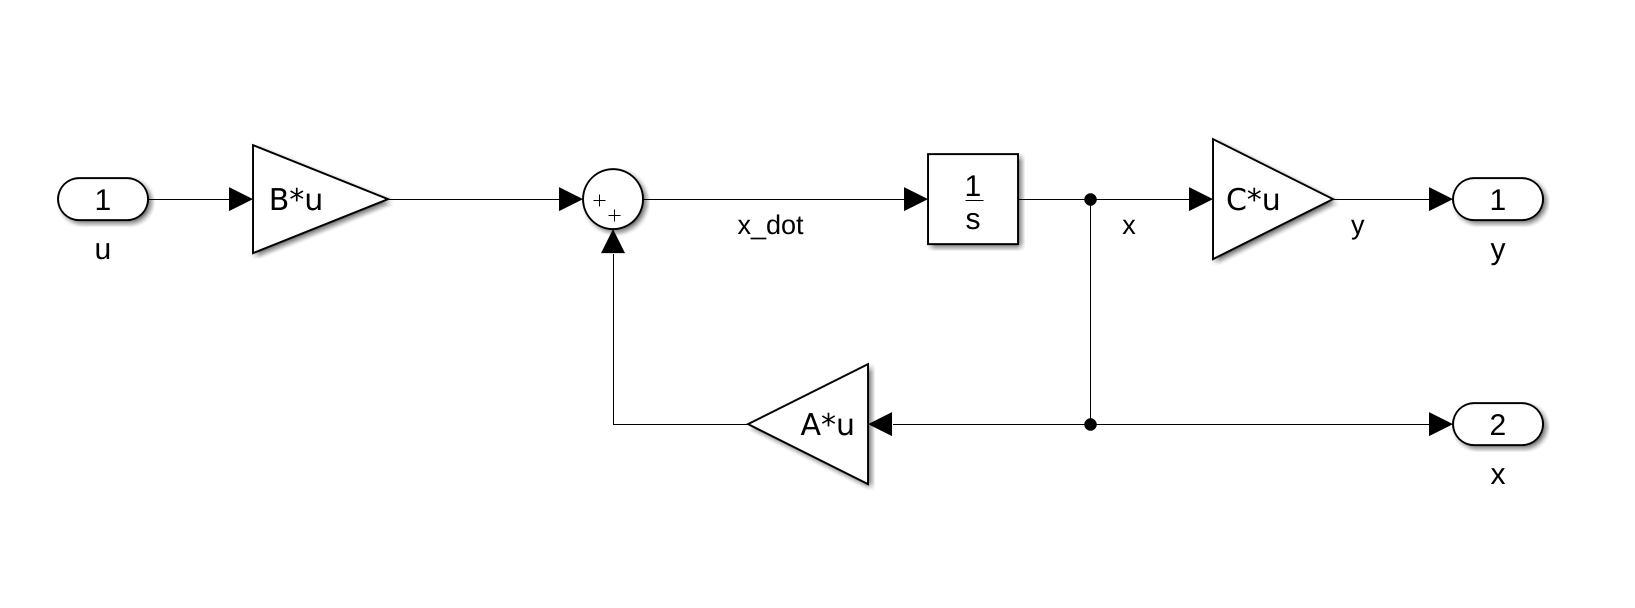
\includegraphics[width=0.6\textwidth]{plant.png}
    \caption{Plant model in Simulink.}
    \label{fig:plant}
\end{figure}

In the Matlab system can be represented by the state space function:
\begin{lstlisting}[frame=single]
>>sys = ss(A,B,C,D)
\end{lstlisting}



\subsection{Open loop response}
The system is stable only if all the real parts of the eigenvalues are
negative. \\
The dynamics of the model is determined by the following parameters:\\
\textbf{Pols:}
\begin{align*}
   0.0000 + 0.0000i \\
  -0.3715 + 0.8938i \\
  -0.3715 - 0.8938i \\
\end{align*}
The real parts of eigenvalues are negative. The system is \textbf{stable}.\\
\textbf{Controllability matrix rank: $3$} \\
If the rank of Controllability matrix $Co = [ B\ AB\ A^2B\ \dots\ A^{n-1}B ]$
is equal to $n$ (number of states), the system is \textbf{controllable}. \\
\textbf{Observability matrix rank: $3$} \\
If the rank of Observability matrix $O = [ C\ CA\ CA^2\ \dots\ CA^{n-1} ]$
is equal to $n$, the system is \textbf{observable}.

The whole system is described by \ref{sys_ss} equations.
Open-loop impulse response is presented on figure
\ref{fig:open_loop_impuls}. The result corresponds to our expectations.

Open-loop step response is presented on figure
\ref{fig:open_loop_step}. The result corresponds to our expectations.
Aircraft started to increase pitch angle.

\begin{figure}[hbt!]
    \centering
    \begin{minipage}{.5\textwidth}
    \centering
    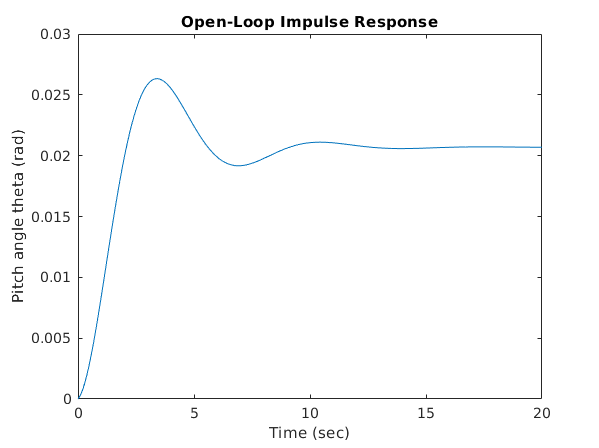
\includegraphics[width=1\textwidth]{open_loop_impuls.png}
    \caption{Open-loop impulse response.}
    \label{fig:open_loop_impuls}
\end{minipage}%
\begin{minipage}{.5\textwidth}
    \centering
    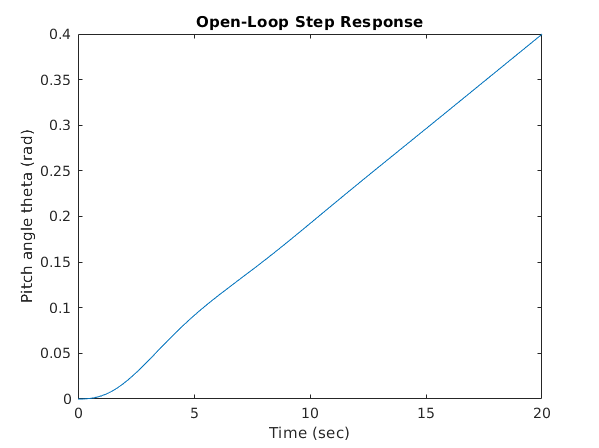
\includegraphics[width=1\textwidth]{open_loop_step.png}
    \caption{Open-loop step response.}
    \label{fig:open_loop_step}
\end{minipage}
\end{figure}


\pagebreak

\subsection{LQR design - zero control}
In modeling zero control response, the input of the system
will be $u = -Kx$, ($r=0$). Substituting into equation \ref{sys_ss}, the
result of Close-loop system will correspond to equation \ref{sys_cl}.

\begin{align}\label{sys_cl}
    \dot{x} = (A-BK)x
\end{align}

For calculation $K$ gain were used LQR method. This method based on quadratic
cost function $J$. Where $Q$ matrix represent how "fast" controller will approximate 
the following state. 
$R$ matrix represent how much we depend on energy that we add to system to
control.
\begin{equation}
J=\int(x^TQx + u^TRu)dt
\end{equation}


In Matlab we define Q and R matrix and use a \textbf{lqr} command.
\begin{lstlisting}[frame=single]
Q = diag([0, 0, 500]);
R = .1;
K = lqr(A,B,Q,R);
\end{lstlisting}

Simulink model of Close-loop system is presented in the following diagram
\ref{fig:zero_control}.

\begin{figure}[h]
    \centering
    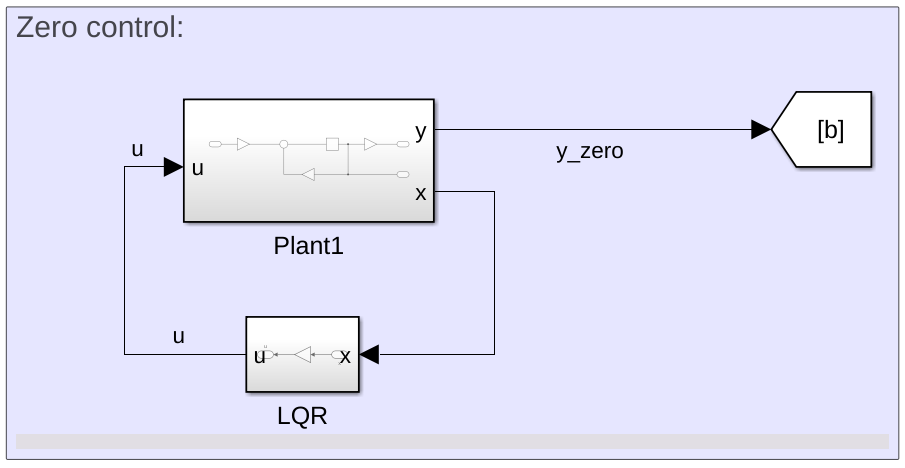
\includegraphics[width=0.6\textwidth]{zero_control.png}
    \caption{Zero control model in Simulink.}
    \label{fig:zero_control}
\end{figure}

\subsection{LQR design - control to the point - rscale}

$N$ gain is used to scalar our input for a full-state feedback system to 
eliminate the steady-state error.
\begin{equation}\label{r_n}
    u = -Kx + rN
\end{equation} 
where $r$ is final point. Substituting equation \ref{r_n} into equation \ref{sys_ss}, the
result of Close-loop system controlled to $r$ will correspond to equation
\ref{BNr}.
\begin{equation}\label{BNr}
    \dot{x} = (A-BK)x + BNr
\end{equation}

For calculation \textbf{N} gain in matlab were used rscale function from
\cite{rscale}. 
\begin{lstlisting}[frame=single]
N = rscale(A,B,C,D,K);
\end{lstlisting}

Simulink model of Close-loop system controled to point is presented in the following diagram
\ref{fig:model_to_point}.

\begin{figure}[hbt!]
    \centering
    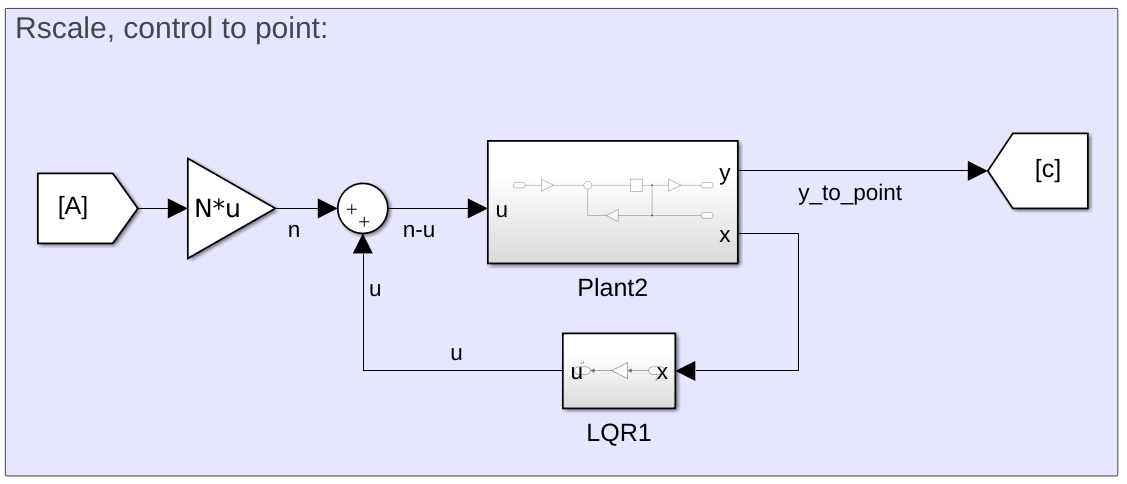
\includegraphics[width=0.6\textwidth]{model_to_point.png}
    \caption{Rscale control to point model in Simulink.}
    \label{fig:model_to_point}
\end{figure}
In the Matlab system can be represented by the state space function:
\begin{lstlisting}[frame=single]
>>sys = ss(A-B*K,B*N,C,D)
\end{lstlisting}

The Close-loop impulse and step response are presented in the following
figure \ref{fig:close_loop_impuls}, \ref{fig:close_loop_step}.

\begin{figure}[hbt!]
    \centering
    \begin{minipage}{.5\textwidth}
    \centering
    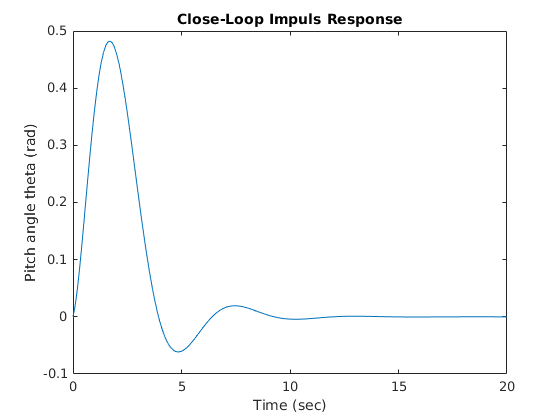
\includegraphics[width=1\textwidth]{close_loop_impuls.png}
    \caption{Close-loop impulse response.}
    \label{fig:close_loop_impuls}
\end{minipage}%
\begin{minipage}{.5\textwidth}
    \centering
    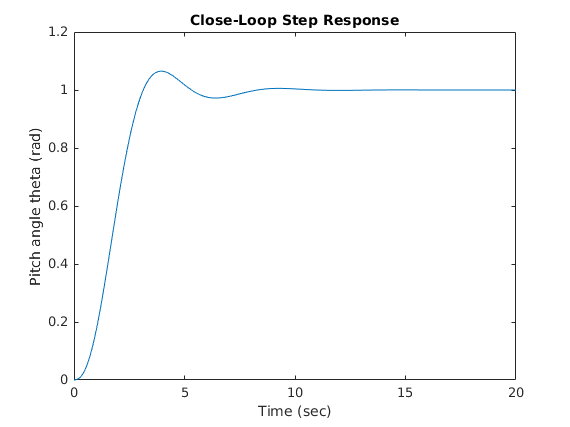
\includegraphics[width=1\textwidth]{close_loop_step.png}
    \caption{Close-loop step response.}
    \label{fig:close_loop_step}
\end{minipage}
\end{figure}
\subsection{Study of system behavior}

In case Longitudinal dynamic it's possible to measure $\theta$ (pitch
angle). There is no specific conditions for deflector angle actuator. The
$R = 0.1$ matrix we will keep equal to 0.1. In the following figure
\ref{fig:diff_Q}, there are impulse responses for 
different $Q$ matrices. Where we change $x$ parameter from 1 to 500 with 50 as
step.


$Q = \begin{bmatrix}  0 & 0 & 0 \\
                      0 & 0 & 0 \\
                      0 & 0 & x \end{bmatrix}$ \\

\begin{figure}[hbt!]
    \centering
    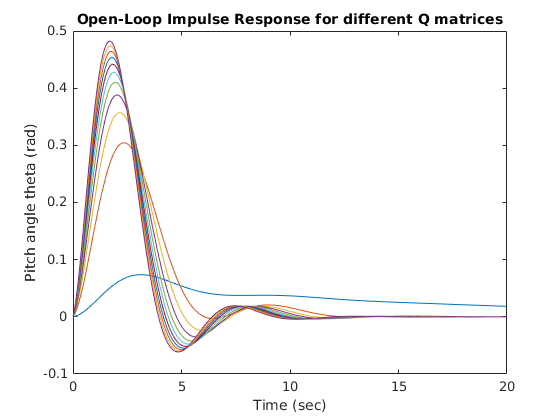
\includegraphics[width=0.6\textwidth]{diff_Q.png}
    \caption{Impulse response for different Q matrices.}
    \label{fig:diff_Q}
\end{figure}
The following Q and R matrices will suffice for our purposes. These values
will be used in the following simulations.

$Q = \begin{bmatrix}  0 & 0 & 0 \\
                      0 & 0 & 0 \\
                      0 & 0 & 500 \end{bmatrix}$  \
$R = 0.1$


\subsection{Observer's proposal}
The LQR controller can be used if we have information about the whole
state $x$. A Kalman filter can be used to reconstruct the state from the
$y$ measurement. The following system of equations \ref{kf} representing Kalman filter.

\begin{equation}\label{kf}
    \begin{split}
        \frac{d}{dt}\hat{x} = A\hat{x} + Bu + Kf(y-\hat{y})\\
        \hat{y} = C\hat{x}
    \end{split}
\end{equation}


Simulink model of Kalman filter is presented in the following diagram
\ref{fig:kf_model}.

\begin{figure}[hbt!]
    \centering
    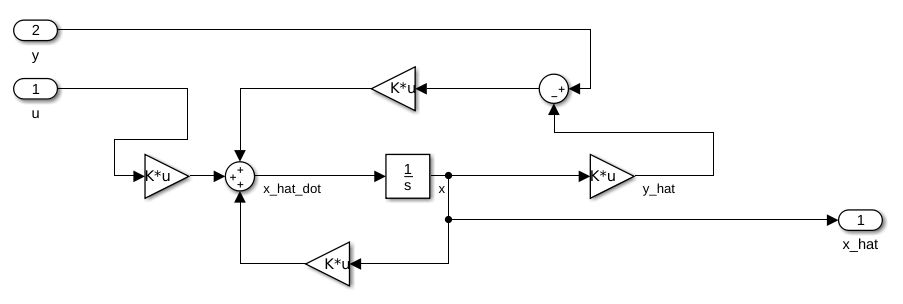
\includegraphics[width=0.6\textwidth]{kf_model.png}
    \caption{Kalman filter implementation in Simulink}
    \label{fig:kf_model}
\end{figure}

Kalman filter use knowledge  about disturbance of state and measurement
noise magnitudes. $Vd$ matrix representing covariance of state disturbance
and $Vn$ matrix is covariance of measurement noise.
There are more options how to calculate $Kf$ gain. Define $Vd$
and $Vn$ matrices we can use the same \textbf{lqr} function as follow: 

\begin{lstlisting}[frame=single]
Vd = .01*eye(3); 
Vn = 1;
Kf = (lqr(A',C',Vd,Vn))';
\end{lstlisting}

Simulink model of system is presented in the following diagram
\ref{fig:lqg}.

\begin{figure}[hbt!]
    \centering
    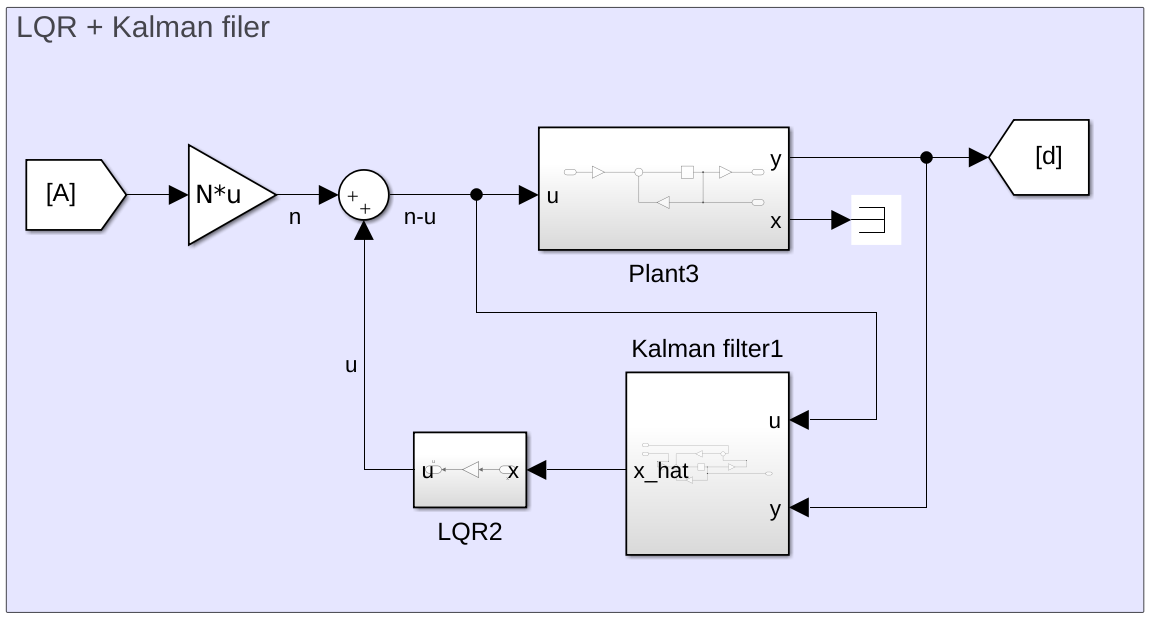
\includegraphics[width=0.6\textwidth]{model_lqr_kalman.png}
    \caption{Rscale control to point model in Simulink.}
    \label{fig:lqg}
\end{figure}

Implementing Kalman filter in Matlab:
\begin{lstlisting}[frame=single]
Akf = A-Kf*C;
Bkf = [B Kf];
Ckf = eye(3);
Dkf = 0*[B Kf];
sys_kf = ss(Akf, Bkf, Ckf, Dkf);
\end{lstlisting}

\subsection{Study of system behavior with an observer (simulation)}
The real system control contain measurement noise and disturbance. In model
\ref{fig:lqg_noise} were used $w_d$ and $w_n$ disturbance and noise inputs
as Gaussian white noise.


The whole system with LQG implementation, disturbances and noise can be
describe as following system of equations \ref{lqg_final}.
\begin{equation}
        \epsilon = x - \hat{x} \\
\end{equation}


\begin{equation}\label{lqg_final}
\begin{bmatrix} \dot{x} \\ \dot{\epsilon} \end{bmatrix}  = 
\begin{bmatrix} A-BK & BK \\ 0 & A-KfC \end{bmatrix} \cdot 
\begin{bmatrix} x \\ \epsilon \end{bmatrix} +
\begin{bmatrix} I & 0 \\
                I & -Kf
\end{bmatrix} \cdot
\begin{bmatrix} w_d \\ w_n \end{bmatrix}
\end{equation}

The whole model is controlled by placing eigenvalues in $A-BK$ and $A-KfC$
by $K$ and $Kf$ matrices. 
 

Simulink model is presented in the following diagram
\ref{fig:lqg_noise}.

\begin{figure}[hbt!]
    \centering
    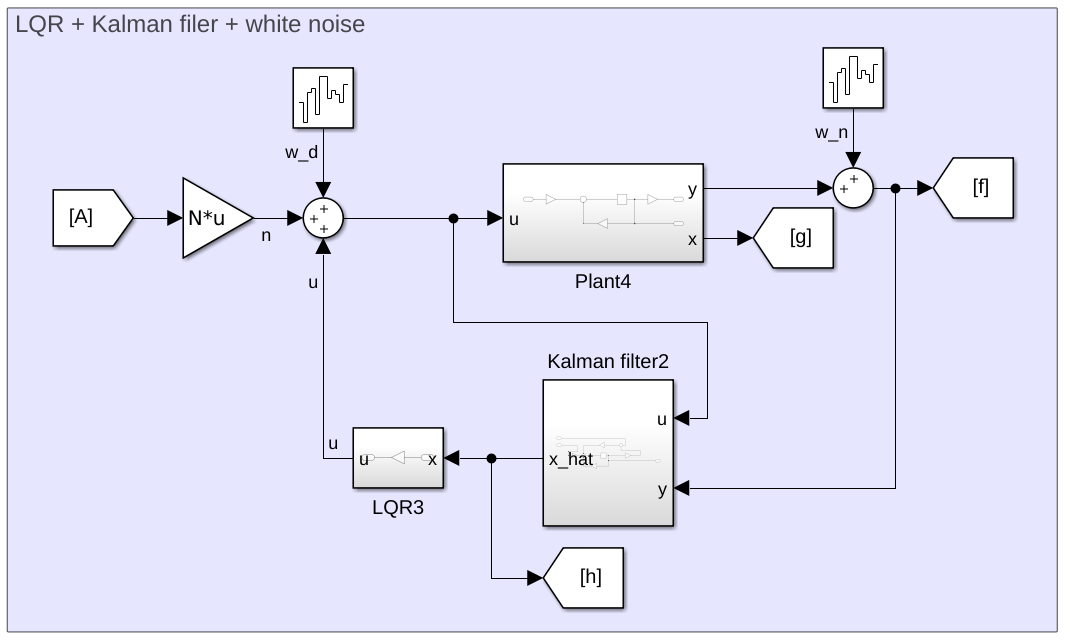
\includegraphics[width=0.6\textwidth]{lqg_noise.png}
    \caption{LQG simulink model}
    \label{fig:lqg_noise}
\end{figure}


The following graph \ref{fig:lqg_noise_plot} shows the correct operation
of the LQG controller. Kalman filter correctly estimates the state with
permissible noise level.

\begin{figure}[hbt!]
    \centering
    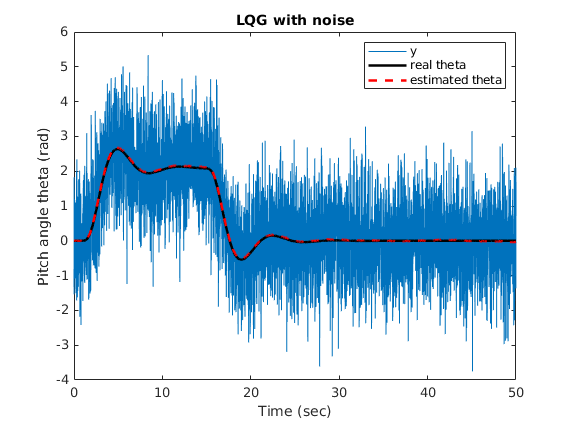
\includegraphics[width=0.6\textwidth]{lqg_noise_plot.png}
    \caption{LQG regulator output}
    \label{fig:lqg_noise_plot}
\end{figure}

With increasing noise amplitude, the model is able to remain functional.
This can be verified by changing the disturbance and noise magnitude in the
Simulink model.

\subsection{Evaluation of the whole task and conclusion}

LQG can be used to control the pitch angle of an aircraft. LQG is
sufficiently resistant to the disturbance and measurement noise.
Implementation in the Matlab/Simulink environment sufficiently clear and
easily scalable.
All Simulink models and Matlab scripts are available in appendix.


\end{document}
